%%%%%%%%%%%%%%%%%%%%%%%%%%%%%%%%%%%%%%%%%%%%%%%%%%%%%%%%%%%%%%%%%%%%%%%%%%%%%%%%%%%%%%%%%%%%%%%%%%%%%%%%%%%%%%%%%

\UC{Ordinamento prodotti PLP per ordine alfabetico}
\label{ordinamento-alfabetico}

L'utente non autenticato o l'acquirente può ordinare i prodotti risultanti dalla ricerca effettuata in precedenza per ordine alfabetico.
\begin{itemize}
    \item \textbf{Attori primari:} acquirente o utente non autenticato;
    \item \textbf{Precondizione:} l'attore è nella PLP e ha selezionato l'ordinamento per ordine alfabetico;
    \item \textbf{Postcondizione:} i prodotti nella schermata vengono ordinati in ordine alfabetico;
    \item \textbf{Scenario principale:} l'attore vuole ordinare i prodotti nella schermata così da averli elencati in ordine alfabetico.
\end{itemize}

%%%%%%%%%%%%%%%%%%%%%%%%%%%%%%%%%%%%%%%%%%%%%%%%%%%%%%%%%%%%%%%%%%%%%%%%%%%%%%%%%%%%%%%%%%%%%%%%%%%%%%%%%%%%%%%%%

\UC{Ordinamento prodotti PLP per prezzo crescente}
\label{ordinamento-prezzo-crescente}

L'utente non autenticato o l'acquirente può ordinare i prodotti risultanti dalla ricerca effettuata in precedenza per prezzo crescente.
\begin{itemize}
    \item \textbf{Attori primari:} acquirente o utente non autenticato;
    \item \textbf{Precondizione:} l'attore è nella PLP e ha selezionato l'ordinamento per prezzo crescente;
    \item \textbf{Postcondizione:} i prodotti nella schermata vengono ordinati in ordine di prezzo crescente;
    \item \textbf{Scenario principale:} l'attore vuole ordinare i prodotti nella schermata così da averli elencati dal più economico al più costoso.
\end{itemize}

%%%%%%%%%%%%%%%%%%%%%%%%%%%%%%%%%%%%%%%%%%%%%%%%%%%%%%%%%%%%%%%%%%%%%%%%%%%%%%%%%%%%%%%%%%%%%%%%%%%%%%%%%%%%%%%%%

\UC{Ordinamento prodotti PLP per prezzo decrescente}
\label{ordinamento-prezzo-decrescente}

L'utente non autenticato o l'acquirente può ordinare i prodotti risultanti dalla ricerca effettuata in precedenza per prezzo decrescente.
\begin{itemize}
    \item \textbf{Attori primari:} acquirente o utente non autenticato;
    \item \textbf{Precondizione:} l'attore è nella PLP e ha selezionato l'ordinamento per prezzo decrescente;
    \item \textbf{Postcondizione:} i prodotti nella schermata vengono ordinati in ordine di prezzo decrescente;
    \item \textbf{Scenario principale:} l'attore vuole ordinare i prodotti nella schermata così da averli elencati dal più costoso al più economico.
\end{itemize}

%%%%%%%%%%%%%%%%%%%%%%%%%%%%%%%%%%%%%%%%%%%%%%%%%%%%%%%%%%%%%%%%%%%%%%%%%%%%%%%%%%%%%%%%%%%%%%%%%%%%%%%%%%%%%%%%%

\UC{Aggiunta al carrello dalla PLP}
\label{aggiunta-carrello-plp}

\begin{figure}[H]
    \centering
    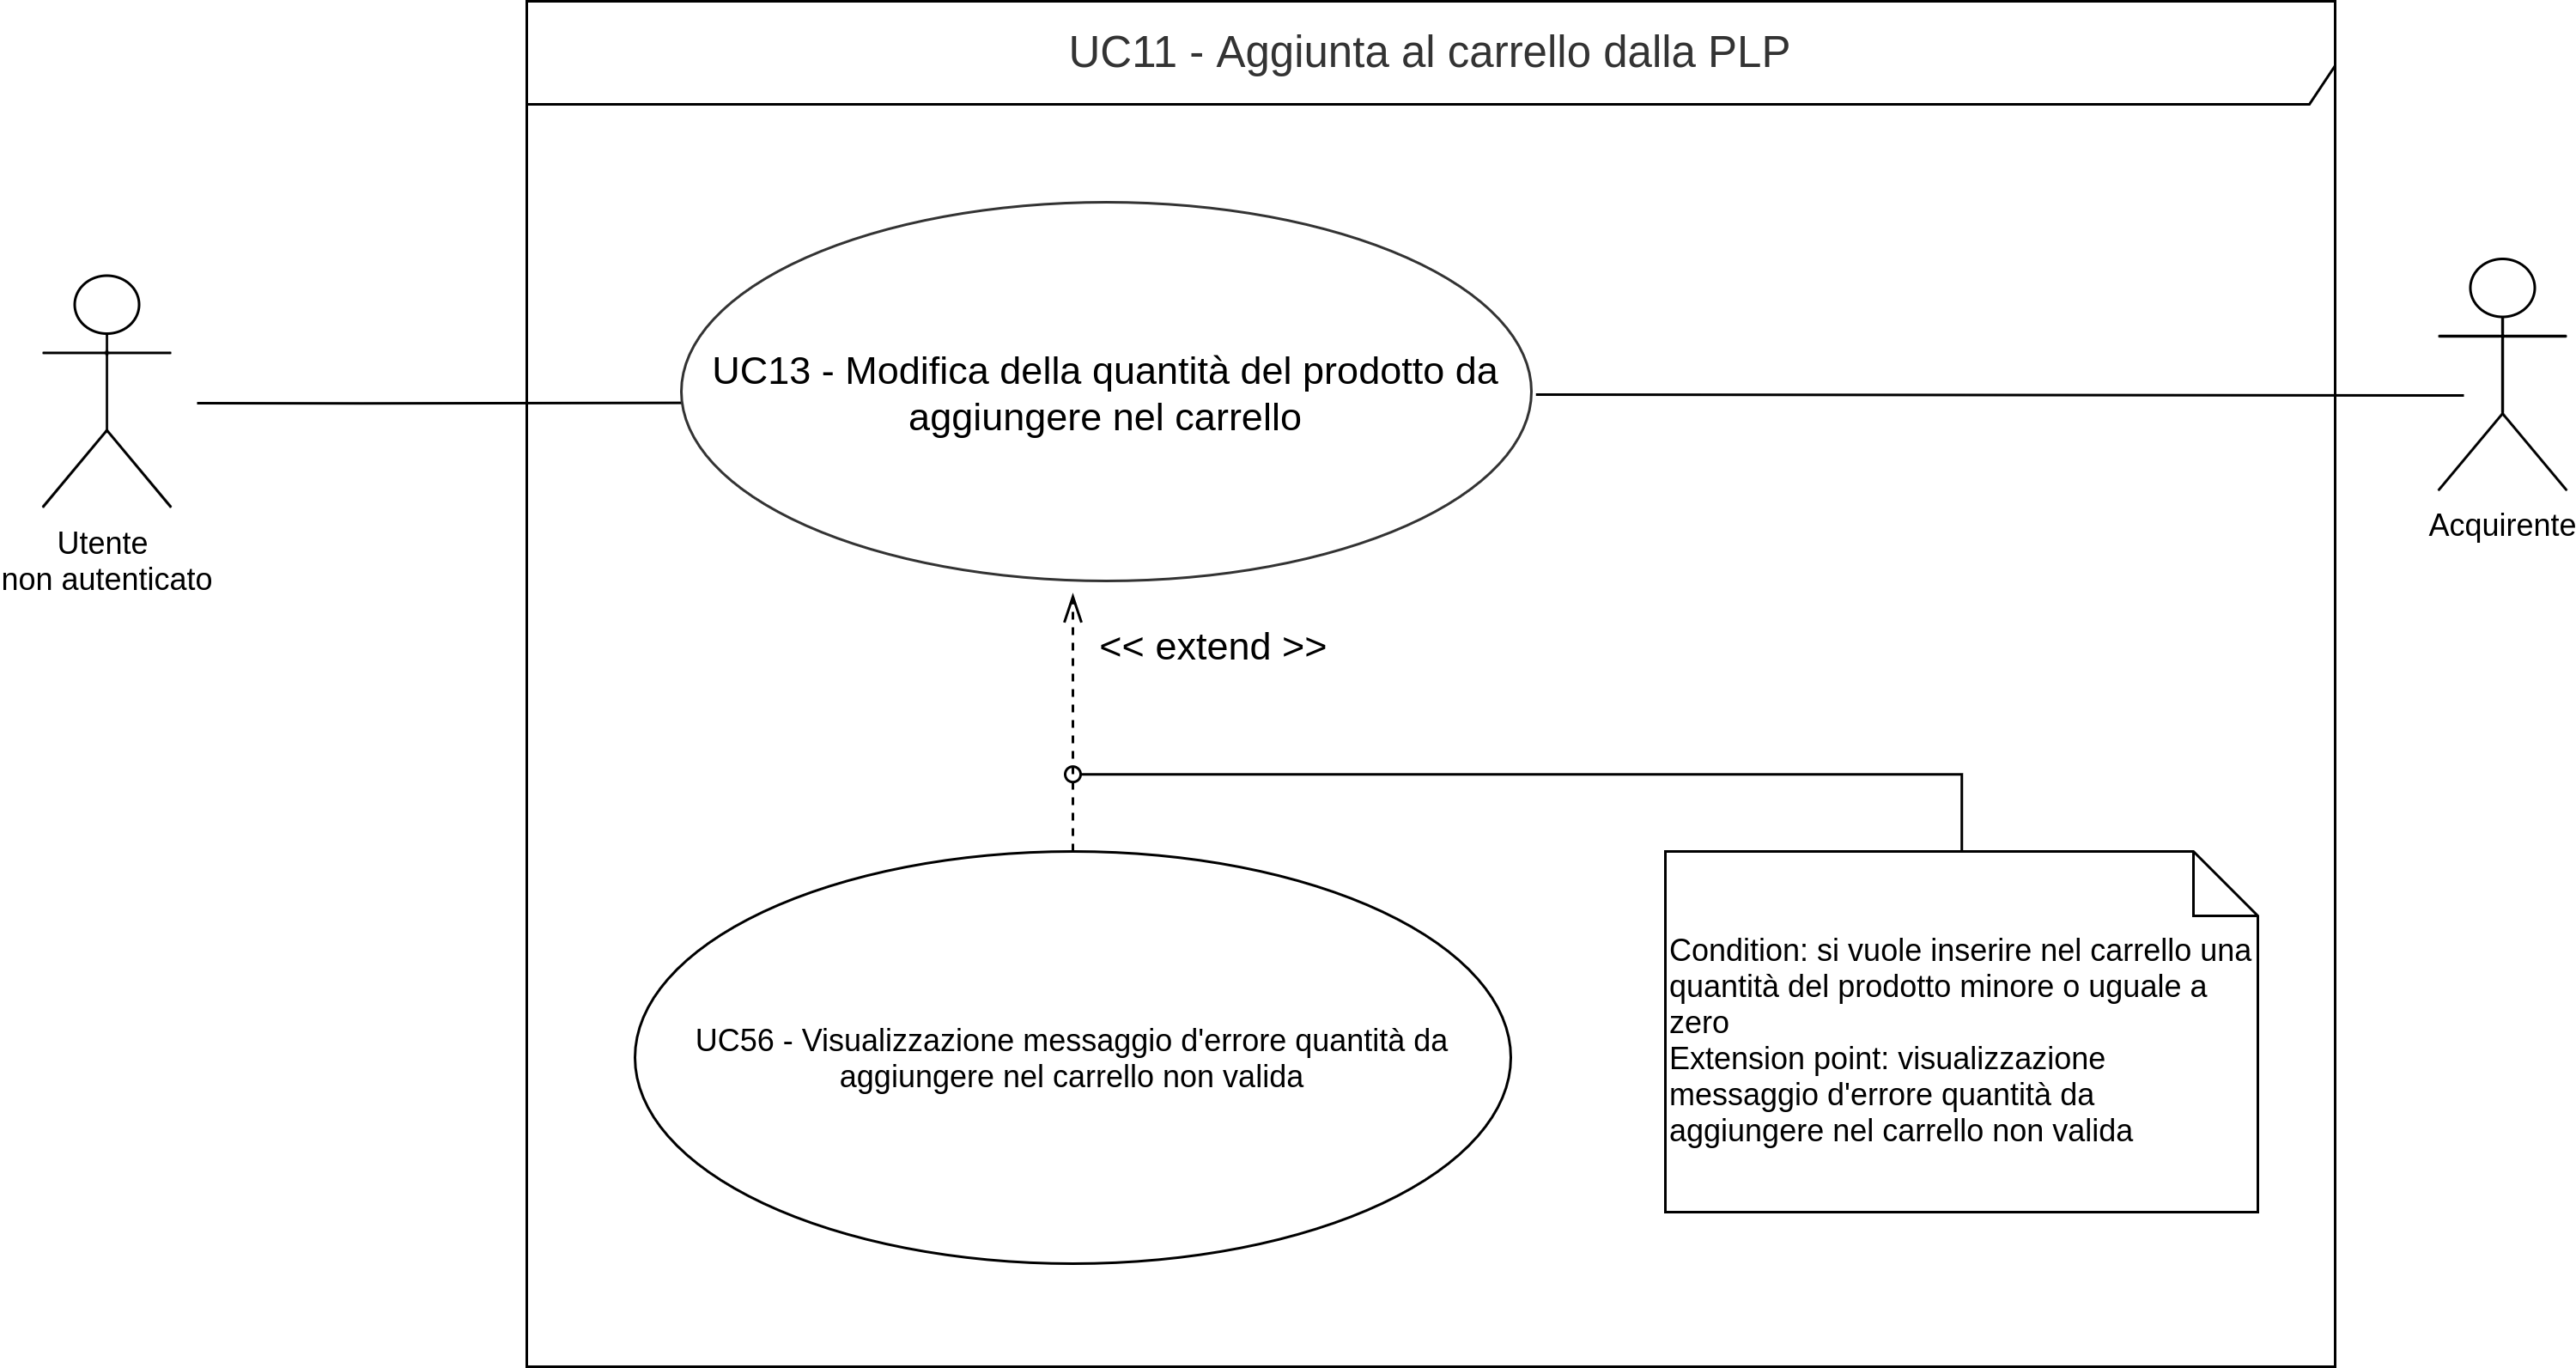
\includegraphics[scale=0.4]{Immagini/DiagrammiUC/Acquirente/AggiuntaProdottiCarrelloPLP.png}
    \caption{Diagramma di \actualUC: Aggiunta al carrello dalla PLP}
    \label{fig:aggiunta-carrello-plp}
\end{figure}

L'utente non autenticato o l'acquirente può aggiungere al carrello i prodotti direttamente dalla PLP.
\begin{itemize}
    \item \textbf{Attori primari:} acquirente o utente non autenticato;
    \item \textbf{Precondizione:} l'attore si trova nella PLP;
    \item \textbf{Postcondizione:} l'attore rimane nella PLP ed al carrello è stato aggiunto il prodotto nella quantità desiderata;
    \item \textbf{Scenario principale:} l'attore vuole aggiungere al carrello un prodotto visualizzato nella PLP e in tal caso:
    \begin{itemize}
        \item (UC\ref{modifica-quantita-da-aggiungere-al-carrello}) - Modifica la quantità del prodotto da aggiungere nel carrello;
        \item Seleziona la funzione di aggiunta al carrello del seguente prodotto nella quantità impostata.
    \end{itemize}
\end{itemize}